% !TEX root = ../Thesis.tex

\chapter{Polimorfismo}
Il polimorfismo è un concetto fondamentale della programmazione. Derivato dal greco “molte forme”, il polimorfismo consente a entità di assumere diverse forme o comportamenti in base al contesto, permettendo di scrivere codice più flessibile, estendibile e manutenibile. Grazie al polimorfismo, è possibile utilizzare un'interfaccia comune per manipolare elementi di tipi diversi, facilitando così l'implementazione di soluzioni generiche. Il vantaggio principale del polimorfismo è il miglioramento della qualità del codice:
\begin{itemize}
    \item Favorisce l'astrazione, consentendo di trattare oggetti di tipi diversi in modo uniforme.
    \item Riduce la duplicazione di codice, poiché le operazioni comuni possono essere definite una sola volta e riutilizzate per diversi tipi.
    \item Semplifica la gestione delle estensioni future, poiché nuove funzionalità possono essere aggiunte senza modificare il codice esistente.
\end{itemize}
In un linguaggio come Java, orientato agli oggetti, il polimorfismo è una caratteristica centrale e largamente supportata tramite ereditarietà e interfacce. Rust, pur non essendo un linguaggio tradizionalmente orientato agli oggetti, offre un approccio alternativo al polimorfismo, basato su trait (tratto, nel senso di caratteristica) e tipi generici, che permette di ottenere astrazione e flessibilità.

In questo capitolo verrà fornita una panoramica delle modalità con cui Java e Rust implementano e sfruttano il polimorfismo, confrontando i due linguaggi.

\section{Polimorfismo in Java}
Java supporta il polimorfismo attraverso due principali meccanismi: il \textit{subtyping} (polimorfismo per inclusione) e il \textit{parametric polymorphism} (polimorfismo parametrico). 

Il subtyping si basa sul fatto che ci possa essere una relazione tra tipi chiamata \textit{relazione di sottotipo}. Si dice che un tipo \textit{A} è un sottotipo di un tipo \textit{B} quando il contesto richiede un elemento di tipo \textit{B} ma può accettare un elemento di tipo \textit{A}. In Java, la relazione di sottotipo viene implementata attraverso l'ereditarietà e le interfacce. Le classi possono estendere altre classi e implementare interfacce, consentendo agli oggetti di essere trattati come istanze della loro classe base o interfaccia. 

Il parametric polymorphism permette di assegnare a una parte di codice un tipo generico, utilizzando variabili di tipo al posto di tipi specifici, che poi possono essere istanziate con tipi concreti al momento dell'utilizzo. In particolare, Java supporta anche:
\begin{itemize}
    \item il \textit{bounded parametric polymorphism}, che consente di specificare vincoli sui parametri di tipo.
    \item il \textit{F-bounded polymorphism} \cite{greenman-effing-bound-polymorphism}, che è la capacità di poter definire vincoli su un tipo generico che dipendono da quel tipo stesso. In altre parole, avere un vincolo di tipo ricorsivo. Ad esempio \texttt{<T extends Comparable<T>}\texttt{>}.
\end{itemize}
\section{Polimorfismo in Rust}
In Rust, il polimorfismo è implementato attraverso i concetti di \textit{trait} e i \textit{generics}. I trait sono simili alle interfacce in Java e definiscono un insieme di metodi che un tipo deve implementare per essere considerato conforme a quel trait. I generics consentono di scrivere funzioni e strutture dati che possono operare su tipi diversi senza dover specificare un tipo concreto. Tramite l'uso dei generics si ottiene il \textit{parametric polymorphism}, mentre attraverso i trait si ottiene il \textit{bounded parametric polymorphism}.\footnote{Entrambe le forme di polimorfismo hanno la stessa definizione data in precedenza per Java.}
\section{Generics: Monomorphization e Type Erasure}
\label{sec:generics}
Sia Rust che Java supportano la programmazione generica, che consente di scrivere codice che può operare su tipi diversi senza avere codice duplicato per ogni tipo specifico. La sintassi per definire i generics in Rust e Java è simile: si utilizzano parentesi angolari per specificare i parametri di tipo. Tuttavia, ci sono differenze significative nella gestione dei generics tra i due linguaggi.

Il compilatore Java utilizza un processo chiamato \textit{type erasure} per implementare i generics, questo include i seguenti fatti:
\begin{itemize}
    \item Durante la compilazione i parametri di tipo vengono sostituiti con il tipo \texttt{Object} o con un tipo specifico se è stato definito un vincolo sul parametro di tipo.
    \item Vengono inseriti cast espliciti per mantenere la type safety.
    \item Generazione di \textit{Bridge Methods} per preservare il polimorfismo dopo il processo di type erasure.
\end{itemize}
Ad esempio:
\begin{minted} [fontsize=\small] {Java}
    public class GenericClass<T> {
        T value;

        void setValue(T value) { 
            this.value = value;
        }
    }
\end{minted}
Dopo la type erasure, il codice diventa:
\begin{minted} [fontsize=\small] {Java}
    public class GenericClass {
        Object value;

        void setValue(Object value) { 
            this.value = value;
        }
    }
\end{minted}
Nel caso in cui, invece, si definisca un vincolo di tipo, ad esempio \texttt{<T extends Number>}, il compilatore Java sostituirà \texttt{T} con \texttt{Number} durante la type erasure, mantenendo la type safety:
\begin{minted} [fontsize=\small] {Java}
    public class GenericClass{
        Number value;

        void setValue(Number value) { 
            this.value = value;
        }
    }
\end{minted}
Quando si combina la type erasure con l'overriding dei metodi, Java genera dei \textit{Bridge Methods} per garantire che il polimorfismo funzioni correttamente. Uno scenario tipico è il seguente:
\begin{itemize}
    \item Una classe generica o un'interfaccia ha un metodo che usa un tipo generico. 
    \item Una sua sottoclasse sovrascrive quel metodo con un tipo concreto. 
    \item Dopo la type erasure, le firme dei due metodi non corrispondono più. Questo romperebbe il polimorfismo. 
\end{itemize}
Ad esempio: 
\begin{minted} [fontsize=\small] {Java}
    class Parent<T> {
        T getValue() { return null; }
    }

    class Child extends Parent<String> {
        @Override
        String getValue() {
             return "Hello"; 
        }
    }
\end{minted}
Dopo la type erasure:
\begin{minted} [fontsize=\small] {Java}
    class Parent {
        Object getValue() {
            return null; 
        }
    }

    class Child extends Parent {
        String getValue() {
            return "Hello"; 
        }

        // Bridge method generato dal compilatore:
        // Garantisce che la chiamata a Parent.getValue() 
        // funzioni correttamente
        Object getValue() {
            return this.getValue(); // chiama String getValue()
        }
    }
\end{minted}
In Rust, invece, i generics sono implementati tramite un processo chiamato \textit{monomorphization}. Questo è il processo tramite cui il compilatore Rust genera codice specifico per ogni tipo concreto utilizzato con i generics. Questo significa che Rust sostituisce i parametri di tipo generici con i tipi concreti utilizzati, e genera una versione specifica della funzione o della struttura per ogni tipo. Ad esempio: 
\begin{minted} [fontsize=\small] {Rust}
    struct Boxed<T> {
        value: T,
    }

    fn main() {
        let a = Boxed { value: 123 }; // T = i32
        let b = Boxed { value: "text" }; // T = &str
    }
\end{minted}
Dopo la monomorphization, il compilatore Rust genera due versioni della struttura \texttt{Boxed}:
\begin{minted} [fontsize=\small] {Rust}
    struct Boxed_i32 {
        value: i32,
    }

    struct Boxed_str {
        value: &str,
    }
\end{minted}
È facile notare come i due approcci siano molto diversi e abbiano implicazioni diverse sul modo in cui il codice viene generato e sulla performance:
\begin{itemize}
    \item Rispetto alla type erasure di Java, la monomorphization di Rust porta diversi vantaggi in termini di performance:
    \begin{itemize}
        \item Nella type erasure, poiché i parametri di tipo vengono eliminati, il compilatore spesso deve inserire cast espliciti per garantire la type safety, il che può introdurre un overhead. Questo overhead è spesso trascurabile ma comunque presente. 
        \item I generics di Java non possono essere utilizzati con tipi primitivi, come \texttt{int} o \texttt{double}, ma solo con oggetti. Questo significa che quando si usano generics con tipi primitivi, Java deve utilizzare il boxing e l'unboxing, che introducono un ulteriore overhead.
        \item Poiché Java usa lo stesso bytecode per tutte le istanziazioni di un generico, non può ottimizzare il codice per tipi specifici. Questo può essere rilevante per sistemi che richiedono un alto grado di performance.
        \item Il monomorphization è un meccanismo statico che risolve i tipi al momento della compilazione, quindi non ha overhead a runtime. Invece, la type erasure può coinvolgere il dynamic dispatch di Java che può essere più costoso in termini di performance.
    \end{itemize}
    \item La monomorphization può portare ad un aumento della dimensione del codice del programma compilato poiché vengono generate diverse versioni della stessa funzione generica, una per ogni combinazione di tipi con cui viene chiamata. 
    \item La monomorphization può incrementare notevolmente il tempo di compilazione del programma, specialmente se ci sono molte combinazioni di tipi concreti con cui viene chiamata una funzione generica.
    \item La monomorphization può fornire messaggi di errore più chiari e specifici poiché ogni versione specifica della funzione generica ha tipi concreti associati.
\end{itemize}
\section{Traits}
\label{sec:rust_traits}
Un \textit{trait} è un costrutto di Rust che consente di definire un insieme di funzionalità che un tipo deve implementare. I traits vengono utilizzati, quindi, per definire comportamenti comuni che possono essere condivisi tra diversi tipi. Questo significa che tutti i tipi che implementano un determinato trait condividono la stessa interfaccia di quel trait. Un trait viene dichiarato utilizzando la keyword \texttt{trait} come segue:
\begin{minted} [fontsize=\small] {Rust}
    pub trait MyTrait {
        fn my_method(&self) -> String;
    }
\end{minted}
L'implementazione del trait avviene attraverso le keywords \texttt{impl} e \texttt{for} come segue:
\begin{minted} [fontsize=\small] {Rust}
    struct MyStruct;

    impl MyTrait for MyStruct {
        fn my_method(&self) -> () {
            println!("Hello from MyStruct");
        }
    }
\end{minted}
I traits possono essere utilizzati per realizzare il bounded parametric polymorphism in Rust, consentendo di specificare vincoli sui tipi generici (\textit{trait bounds}). Ad esempio, si può definire una funzione che accetta un tipo generico che implementa un determinato trait nel seguente modo:
\begin{minted} [fontsize=\small] {Rust}
    fn my_function<T: MyTrait>(item: T) {
        println!("{}", item.my_method());
    }
\end{minted}
Nel caso in cui siano presenti più vincoli, questi possono essere combinati utilizzando il simbolo \texttt{+} oppure attraverso l'uso di \texttt{where}:
\begin{minted} [fontsize=\small] {Rust}
    fn my_function<T>(item: T)
    where 
        T: MyTrait + AnotherTrait 
    {
        println!("{}", item.my_method());
    }   
\end{minted}
In Java, è possibile ottenere un comportamento simile ai trait bounds attraverso i vincoli di tipo (\textit{type bounds}) nelle dichiarazioni generiche. Ad esempio, si può definire una classe generica che accetta un tipo che estende una classe base o implementa un'interfaccia:
\begin{minted} [fontsize=\small] {Java}
    public class MyClass<T extends Bound> {
        /* ... */
    }
\end{minted}
In questo esempio, \texttt{T} è un tipo generico che deve implementare \texttt{Bound}. Questo consente di utilizzare i metodi definiti in \texttt{Bound} all'interno della classe \texttt{MyClass}. Anche in Java è possibile definire più vincoli di tipo\footnote{A causa dell'ereditarietà singola di Java solo un vincolo può essere una classe: il primo nella lista.} attraverso l'utilizzo dell'operatore \texttt{\&}:
\begin{minted} [fontsize=\small] {Java}
    public class MyClass<T extends Bound & AnotherBound> {
        /* ... */ 
    }
\end{minted}
Si può facilmente notare come il concetto di trait in Rust sia molto simile alle interfacce in Java. Entrambi servono entrambi a garantire che un valore o un oggetto possa essere utilizzato secondo un certo protocollo o insieme di regole, permettendo diverse implementazioni concrete senza essere vincolati a dettagli di implementazione, a differenza di quanto accade con una superclasse Java. Tuttavia, sono presenti alcune differenze significative:
\begin{itemize}
    \item In Rust, un trait non è un tipo concreto, ma un insieme di metodi che un tipo può implementare. In Java, invece, un' interfaccia funge sia da contratto sia da tipo: quando una classe implementa un'interfaccia, è possibile trattare gli oggetti di quella classe come istanze del tipo dell'interfaccia stessa. La differenza principale è, quindi, che in Rust il trait è separato dal tipo concreto, mentre in Java l'interfaccia può essere usata direttamente come tipo del riferimento.
    \item In Java, le interfacce richiedono che la classe che le implementa abbia metodi con nomi specifici. Questo può creare conflitti: ad esempio, due interfacce potrebbero essere impossibili da implementare contemporaneamente se hanno metodi con lo stesso nome ma tipi di ritorno diversi. Ad esempio:
    \begin{minted} [fontsize=\small] {Java}
        public interface InterfaceA {
            String getValue();
        }

        public interface InterfaceB {
            int getValue();
        }

        public class MyClass implements InterfaceA, InterfaceB {
            // Errore: il compilatore non sa quale
            // metodo getValue() implementare
        }
    \end{minted}
    In Rust, invece, ogni trait ha il proprio namespace separato. Quando si implementa un trait per un tipo, lo si fa in un blocco \texttt{impl} separato specificando il trait. In questo modo è sempre esplicito a quale trait appartiene ogni metodo, evitando conflitti tra trait diversi. Nel caso in cui  entrambi i trait sono nello scope è necessario specificare il trait usando la sintassi \texttt{Trait::method(\&obj)} invece della semplice chiamata con la notazione puntata.
    \item In Java, le interfacce possono avere parametri di tipo. Tuttavia, un oggetto può implementare un'interfaccia generica solo una volta:
    \begin{minted} [fontsize=\small] {Java}
        public interface anInterface<T> {
            void doSomething(T value);
        }

        public class MyClass implements anInterface<String>,
                                        anInterface<Integer>
        {
            @Override
            public void doSomething(String value) { /* ... */ }
            //Errore: il compilatore non sa quale metodo 
            // doSomething() implementare
        }        
    \end{minted}
    In Rust, invece, un trait generico può essere implementato per molti tipi diversi, e ciascuna implementazione è considerata sostanzialmente un trait distinto:
    \begin{minted} [fontsize=\small] {Rust}
        trait MyTrait<T> {
            fn do_something(&self, value: T);
        }

        struct MyStruct;

        impl MyTrait<String> for MyStruct {
            fn do_something(&self, value: String) { /* ... */ }
        }

        impl MyTrait<i32> for MyStruct {
            fn do_something(&self, value: i32) { /* ... */ }
        }
    \end{minted}
    \item In Rust, è possibile implementare traits per tipi esterni, definiti in altri crate. Questo consente di esterndere il comportamento di tipi che non sono stati definiti nel proprio codice. Questo può essere fatto rimanendo conforme alla \textit{Orphan Rule}: si può implementare un trait per un tipo solo se almeno uno dei due (trait o tipo) è definito nel proprio crate. La regola è stata introdotta per evitare conflitti di implementazione quando più crate cercano di implementare lo stesso trait per lo stesso tipo. In Java, invece, non è possibile aggiungere un'interfaccia a un tipo già definito senza modificarne la classe. Quindi non si può implementare un'interfaccia di un tipo su cui non si ha accesso al codice sorgente. Per ottenere un comportamento simile a Rust, si possono utilizzare tecniche come l'utilizzo di classi \textit{Wrapper}. 
\end{itemize}

\begin{comment}
    \item In Rust, esiste la cosiddetta \textit{Orphan Rule}: si può implementare un trait per un tipo solo se almeno uno dei due (trait o tipo) è definito nel proprio crate \footnote{Un crate è un pacchetto di codice Rust.}. Quindi se il trait è definito nel proprio crate, si può implementare per tipi definiti altrove, ad esempio \texttt{String} o \texttt{i32}. In Java, invece, non è possibile aggiungere un'interfaccia a un tipo già definito senza modificarne la classe. Quindi non si può implementare un'interfaccia di un tipo su cui non si ha accesso al codice sorgente. Per ottenere un comportamento simile a Rust, si possono utilizzare tecniche come l'utilizzo di classi \textit{Wrapper}:
        \begin{minted} [fontsize=\small] {Java}
            public interface MyInterface {
                void doSomething();
            }

            public class MyWrapper implements MyInterface {
                private final String value;

                public MyWrapper(String value) {
                    this.value = value;
                }

                @Override
                public void doSomething() { /* ... */ }
            }
        \end{minted}
\end{comment}
\section{Meccanismi di Dispatch}
Quando il codice coinvolge il polimorfismo, sono necessari meccanismi per determinare quale versione specifica di metodo sta venendo effettivamente eseguita. Questo processo prende il nome di \textit{dispatch}. Esistono due forme di dispatch: 
\begin{itemize}
    \item Lo \textit{Static Dispatch}, in cui la risoluzione della chiamata viene risolta a tempo di compilazione.
    \item Il \textit{Dynamic Dispatch}, in cui la risoluzione della chiamata avviene a run-time. 
\end{itemize}
%TODO Inserire un piccolo confronto pro/contro per s/d dispatch

\subsection{Static Dispatch}
In Rust, il meccanismo di static dispatch viene realizzato attraverso \textit{generics} e i \textit{trait bounds}. Quando si utilizza un tipo generico con un trait bound, il compilatore genera una versione specializzata della funzione per ogni tipo concreto utilizzato. Questo processo è noto come \textit{monomorphization} (descritto in dettaglio nella Sezione \ref{sec:generics}). Per mostrare esplicitamente come lo static dispatch venga implementato in Rust consideriamo il seguente codice:
\begin{minted}[fontsize=\small] {Rust}
    trait Drivable {
        fn drive(&self);
    }

    struct Car;
    impl Drivable for Car {
        #[inline(never)]
        fn drive(&self) {
            println!("You are driving a car.");
        }
    }

    struct Motorcycle; 
    impl Drivable for Motorcycle {
        #[inline(never)]
        fn drive(&self) {
            println!("You are driving a motorcycle.");
        }
    }

    struct Boat;
    impl Drivable for Boat {
        #[inline(never)]
        fn drive(&self) {
            println!("You are driving a boat");
        }
    }
\end{minted}
Definiamo la seguente funzione generica con vincolo di tipo:
\begin{minted}[fontsize = \small]{Rust}
    fn static_dispatch<T: Drivable>(t: T) {
        t.drive();
    }
\end{minted}
Ora, all'interno del nostro \texttt{main()} chiamiamo \texttt{static\_dispatch()} con uno dei tre tipi concreti precedentemente definiti:
\begin{minted}[fontsize = \small]{Rust}
    fn main() {
        static_dispatch(Car{});
        static_dispatch(Motorcycle{});
        static_dispatch(Boat{});
    }
\end{minted}
Durante la compilazione, tramite monomorphization, verranno create tre copie della funzione \texttt{static\_dispatch()}: una per ogni tipo con cui è stata chiamata. Questo si può vedere utilizzando i seguenti comandi\footnote{Il primo comando compila il file Rust senza ottimizzazioni e con informazioni di debug dettagliate. Questo è necessario per produrre un eseguibile "leggibile" e completo per il debug. Il secondo comando utilizza LLDB, un debugger per linguaggi come C e Rust, per disassemblare la funzione \texttt{drive} e mostrare i suoi indirizzi di memoria.} dal terminale:
\begin{minted}[fontsize=\small]{bash}
rustc -C opt-level=0 -C debuginfo=2 main.rs
lldb ./main --batch -o "disassemble --name drive" > disassembly.txt
\end{minted}
Il comando genera un file \texttt{disassembly.txt} contenente la disassemblazione delle funzioni \texttt{drive} con i vari tipi, mostrando chiaramente che ogni funzione ha un indirizzo di memoria distinto:

\begin{verbatim}
Car::drive        -> 0x100000a2c
Motorcycle::drive -> 0x100000a64
Boat::drive       -> 0x100000a9c
\end{verbatim}

Questo evidenzia come lo static dispatch risolva la chiamata alla funzione al momento della compilazione, senza alcun overhead a runtime. 

In Java, lo \textit{static dispatch} è realizzato tramite il \textit{method overloading}. In questo meccanismo, più metodi condividono lo stesso nome ma differiscono per la lista dei parametri (numero o tipo). La scelta del metodo corretto viene risolta dal compilatore in base ai tipi statici degli argomenti.

Consideriamo il seguente esempio:

\begin{minted}[fontsize=\small]{java}
public class StaticDispatch {
		
    public double sum(int op1, int op2) {
        return op1 + op2;
    }
	
    public double sum(double op1, double op2) {
        return op1 + op2;
    }
	
    public static void main(String[] args) {
        double x = new StaticDispatch().sum(1, 1);
        double y = new StaticDispatch().sum(1.0, 1.0);
    }
}
\end{minted}

In questo caso, abbiamo due metodi omonimi \texttt{sum}, rispettivamente con parametri di tipo \texttt{int} e \texttt{double}. Durante la compilazione, la chiamata \texttt{sum(1, 1)} viene risolta come invocazione del metodo \texttt{sum(int, int)}, mentre la chiamata \texttt{sum(1.0, 1.0)} come invocazione del metodo \texttt{sum(double, double)}.  

Per osservare cosa accade a livello di bytecode, compiliamo ed utilizziamo il comando:

\begin{minted}[fontsize=\small]{bash}
    javac .\StaticDispatch.java
    javap -c .\StaticDispatch.class > bytecode.txt
\end{minted}

L'output (semplificato) scritto sul file \texttt{bytecode.txt} è il seguente:
\begin{verbatim}
  public static void main(int[]);
    Code:
       0: new           #7    
       3: dup
       4: invokespecial #9    // Method "<init>":()V
       7: iconst_1
       8: iconst_1
       9: invokevirtual #10   // Method sum:(II)D
      12: dstore_1
      13: new           #7    
      16: dup
      17: invokespecial #9    // Method "<init>":()V
      20: dconst_1
      21: dconst_1
      22: invokevirtual #14   // Method sum:(DD)D
      25: dstore_3
      26: return
\end{verbatim}

Possiamo notare che:
\begin{itemize}
    \item Alla riga 9, \texttt{invokevirtual \#10} corrisponde a \texttt{sum:(II)D}, ovvero il metodo con parametri \texttt{int}.
    \item Alla riga 22, \texttt{invokevirtual \#14} corrisponde a \texttt{sum:(DD)D}, ovvero il metodo con parametri \texttt{double}.
\end{itemize}

Queste informazioni provengono dal \textit{constant pool} \footnote{La constant pool contiene le costanti necessarie per l'esecuzione del codice di una specifica classe. In pratica, è una struttura dati a runtime simile a una tabella dei simboli.} del bytecode, dove il compilatore ha già registrato a quale firma di metodo corrisponde ciascuna chiamata. In altre parole, nonostante entrambe le invocazioni utilizzino l'istruzione \texttt{invokevirtual}, a runtime la JVM non ha bisogno di fare alcuna ricerca aggiuntiva: la firma è già stata scelta a compile-time in maniera univoca.

Sebbene in entrambi i linguaggi si parli di \textit{static dispatch}, i meccanismi adottati sono profondamente diversi. In Rust, lo static dispatch si traduce in specializzazione del codice (funzioni distinte generate dal compilatore). In Java, invece, lo static dispatch si traduce in selezione della firma corretta (una voce distinta nel constant pool per ogni metodo). In entrambi i casi, la risoluzione avviene a compile-time e non vi è alcun overhead di dispatch a runtime. 
\subsection{Dynamic Dispatch}
Il meccanismo di generics e trait bounds appena descritto è adatto solamente quando si lavora con tipi omogenei di cui si conosce  il tipo esatto a compile-time. Tuttavia, quando si desidera lavorare con tipi eterogenei o quando il tipo esatto non è noto fino a runtime, è necessario utilizzare il \textit{dynamic dispatch}. 

Il dynamic dispatch in Rust viene realizzato attraverso l'uso di \textit{trait objects}. Un trait object è un puntatore a un tipo che implementa un determinato trait, consentendo di chiamare metodi definiti nel trait senza conoscere il tipo concreto a compile-time. Un trait object si definisce con la sintassi \texttt{Box<dyn Trait>}\footnote{Al posto di \texttt{Box<>} si può utilizzare qualsiasi altro tipo di puntatore. Questo è richiesto perché il compilatore di Rust deve sapere a compile time la dimensione della variabile.}, dove \texttt{Trait} è il trait che si desidera utilizzare. Ad esempio, consideriamo l'implementazione del design pattern Observer: il \texttt{Subject} deve poter mantenere la collezione degli \texttt{Observer}, i quali vanno trattati in maniera uniforme nonostante possano essere di tipi diversi. Per fare ciò, definiamo il trait \texttt{Observer} e le sue implementazioni:
\begin{listing}[H]
    \begin{minted}[fontsize=\small]{Rust}
        trait Observer {
            fn update(&self, data: &str);
        }

        struct ConcreteObserverA;

        impl Observer for ConcreteObserverA {
            fn update(&self, data: &str) {
                println!("ConcreteObserverA received: {}", data);
            }
        }

        struct ConcreteObserverB;

        impl Observer for ConcreteObserverB {
            fn update(&self, data: &str) {
                println!("ConcreteObserverB received: {}", data);
            }
        }
    \end{minted}
    \caption{Implementazione degli Observer.}
    \label{lst:observer}
\end{listing}
Ora, definiamo il \texttt{Subject} che mantiene una lista di \texttt{Observer} come trait objects:
\begin{minted}[fontsize=\small]{Rust}
    struct Subject {
        observers: Vec<Box<dyn Observer>>,
    }

    impl Subject {
        fn new() -> Self {
            Subject {
                observers: Vec::new(),
            }
        }

        fn add_observer(&mut self, observer: Box<dyn Observer>) {
            self.observers.push(observer);
        }

        fn notify_observers(&self, data: &str) {
            for observer in &self.observers {
                observer.update(data);
            }
        }
    }
\end{minted}
Rust implementa il dynamic dispatch tramite una \textit{vtable}. Essenzialmente, una vtable è una struttura generata dal compilatore che contiene puntatori a funzione. In particolare, un trait object è rappresentato internamente come una coppia di puntatori: 
\begin{itemize}
    \item Un puntatore alla vtable corrispondente alla combinazione tra il tipo concreto e il trait implementato.
    \item Un puntatore ai dati del tipo concreto.
\end{itemize}
\begin{figure}[H]
    \centering
    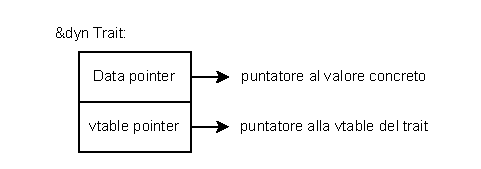
\includegraphics[width=0.8\textwidth]{Figures/vtable.drawio.pdf}
\end{figure}
Va notato che la vtable non è generata per il trait in generale, ma per ciascuna combinazione di tipo concreto e trait implementato. Considerando il listato \ref{lst:observer}, per ogni tipo che implementa il trait \texttt{Observer}, il compilatore genera una vtable separata: quindi sarà presente una vtable per la coppia (\texttt{ConcreteObserverA, Observer}) e una per (\texttt{ConcreteObserverB, Observer}). Quando, all'interno del metodo \texttt{notify\_observers()}, viene chiamato il metodo \texttt{update()} su un trait object, Rust esegue i seguenti passi:
\begin{itemize}
    \item Recupera il puntatore alla vtable del tipo concreto (tranne per \texttt{Object}).
    \item Utilizza il puntatore alla vtable per trovare l'indirizzo della funzione \texttt{update()}.
    \item Chiama la funzione \texttt{update()} passando il puntatore ai dati del tipo concreto.
\end{itemize}
Questo processo consente a Rust di determinare a runtime quale implementazione del metodo chiamare, basandosi sul tipo concreto dell'oggetto. 

In Java, il meccanismo di dynamic dispatch è implementato tramite il \textit{method overriding}, ossia la possibilità di ridefinire un metodo in una sottoclasse. Come in Rust, il metodo da chiamare viene determinato a runtime in base al tipo concreto dell'oggetto. Ogni classe presente in un'applicazione Java ha un'area di memoria all'interno della JVM che contiene metadati riguardanti quel tipo. All'interno di questa area sono contenuti due elementi fondamentali:
\begin{itemize}
    \item Un puntatore alla superclasse.
    \item Un puntatore alla vtable corrispondente al tipo concreto. Questa è simile alla vtable Rust, ossia un puntatore alla tabella dei metodi della classe.
\end{itemize}
In generale, quando viene chiamato un metodo su un oggetto tramite \texttt{invokevirtual}, la JVM consulta la vtable del tipo concreto per determinare quale implementazione del metodo chiamare. Se non esiste una definizione per quel metodo allora la JVM segue il puntatore alla superclasse e riprova finché non viene trovata la definizione del metodo chiamato. 

Per rendere più efficiente l'invocazione dei metodi, le vtable sono organizzate in modo da ridurre al minimo l'overhead dovuto all' attraversamento della gerarchia delle classi. In particolare:
\begin{itemize}
    \item I metodi definiti nella superclasse vengono inseriti nella vtable della sottoclasse nello stesso ordine in cui compaiono nella superclasse.
    \item I nuovi metodi, cioè quelli non presenti nella superclasse, vengono aggiunti in coda alla vtable.
\end{itemize}
Di conseguenza, quando una sottoclasse ridefinisce un metodo, questo mantiene la stessa posizione occupata nella vtable della superclasse, evitando ricerche aggiuntive. Ad esempio, consideriamo la seguente gerarchia di classi:
\begin{figure}[H]
    \centering
    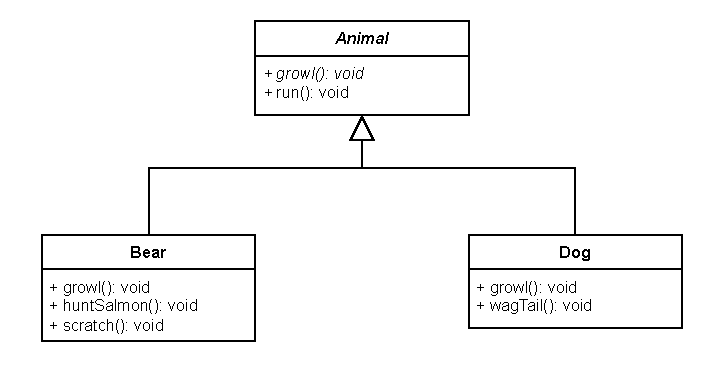
\includegraphics[width=1\textwidth]{Figures/uml1.drawio.pdf}
\end{figure}
Questa produce le seguenti vtable:
\begin{figure}[H]
    \centering
    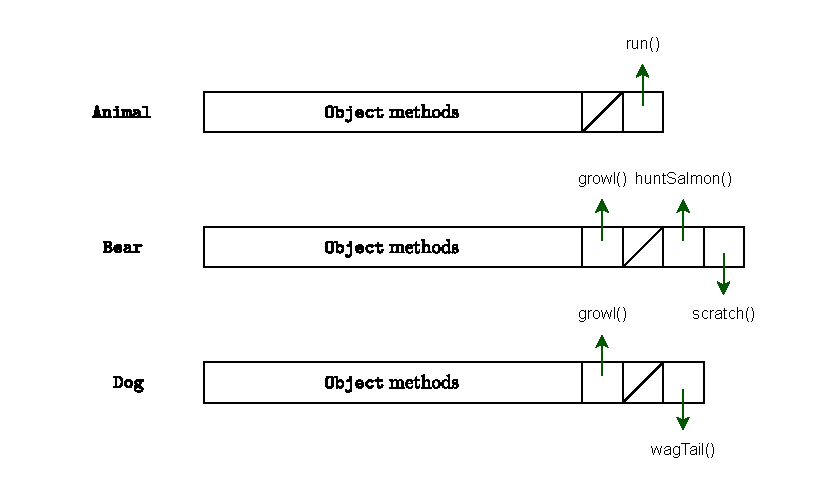
\includegraphics[width=\textwidth]{Figures/vtable1.drawio.pdf}
    \caption{Esempio di vtable in Java.}
    \label{fig:vtable_java}
\end{figure}
Considerando le vtable mostrate in Figura \ref{fig:vtable_java}, quando viene chiamato il metodo \texttt{Bear::run}, la JVM non troverà il metodo sovrascritto nella vtable di \texttt{Bear}, ma seguirà il puntatore alla superclasse \texttt{Animal} dove il metodo è definito \footnote{La prima volta che viene chiamato \texttt{Bear::run} la JVM memorizza il suo indirizzo nella vtable di \texttt{Bear}. In questo modo si migliora la performance delle chiamate successive.}. Nel caso di una gerarchia di classi più profonda, la ricerca potrebbe richiedere più passaggi e diventare più costosa. Da notare che questo sistema funziona solamente perché Java supporta l'ereditarietà singola per le classi: c'è solo un'unica superclasse diretta per ogni tipo (tranne che per \texttt{Object}). 

In conclusione, sia Rust che Java implementano il dynamic dispatch tramite l'uso di vtable, ma con alcune differenze chiave che riflettono i diversi approcci dei due linguaggi al polimorfismo:
\begin{itemize}
    \item In Rust, le vtable sono generate per ogni combinazione di tipo concreto e trait implementato. In Java, invece, ogni classe ha una singola vtable che include tutti i metodi ereditati e quelli definiti nella classe stessa.
    \item In Rust, il dynamic dispatch richiede l'uso esplicito di trait objects (ad esempio \texttt{Box<dyn Trait>}), mentre in Java il dynamic dispatch avviene automaticamente quando si chiama un metodo su un riferimento di tipo superclasse o interfaccia.
    \item Teoricamente, il dynamic dispatch in Rust ha un overhead ridotto rispetto a Java. Questo perché in Rust la vtable viene consultata direttamente per trovare l'indirizzo del metodo, mentre in Java potrebbe essere necessario attraversare la gerarchia delle classi per trovare la definizione del metodo.     
\end{itemize}